\documentclass[12pt,a4paper,oneside]{article} %% Dokumenten Parameter und Art des Dokuments
\usepackage[utf8]{inputenc} %% Diese Datei ist im utf8 Format dies ist hier damit Latex uns versteht
\usepackage[ngerman]{babel} %% Rechtschreib prüfung
\usepackage{hyperref}
\usepackage{amsmath} %% Packet zur verwendung Mathematischer Formeln
\usepackage{amsfonts}
\usepackage{amssymb} %% Packet zur verwendung Mathematischer Symbole
\usepackage{microtype} %% Sorgt für besseren umgang mit zu lange/kurzen Zeilen
\usepackage{pdfpages} %% Zum einfügen eines PDf dokuments
\title{TGI Serie 4}
\author{Bennet Bleßmann, Sven Korfmann}

\begin{document}
\maketitle

\section*{Aufgabe 1}

\subsection*{$L_{1}$)}

$L_{1} = \{w\in\{a,b\}^{*}| |w|_{a} = |w|_{b}\}$

Angenommen ein DEA $m$ existiert mit $p$ Zuständen und $L(m) = L_{1}$.

Dann gilt:

$a^{2p}b^{2p} \in L_{1}$ und somit auch in $L(m)$

Weiter existiert zwangsläufig $x = a^{m}, y = a^{n}, z = a^{2q}b^{2p}$ mit

$n+m+q = 2p$ und $n \geq 1$ und $n+m \leq p$, so dass gilt:

$\forall i \in \mathbb{N}_ : xy^{i}z \in L(m)$

Für $i > 1$ aber ist $xy^{i}z \not\in L_{1}$  

Dies steht im Wiederspruch zur Forderung $L_{1} = L(m)$ und 

ein solches m kann folglich  nicht existieren.

\subsection*{$L_{2}$)}


$L_{2} = \{w\in\{a,b\}^{*}| w = w^{T}\}$

Angenommen ein DEA $m$ existiert mit $p$ Zuständen und $L(m) = L_{2}$.

Dann gilt:

$a^{p+2}ba^{p+2} \in L_{2}$ und somit auch in $L(m)$

Weiter existiert zwangsläufig $x = a^{m}, y = a^{n}, z = a^{q}ba^{p+2}$ mit

$n+m+q = p+2$ und $n \geq 1$ und $n+m \leq p$, so dass gilt:

$\forall i \in \mathbb{N}_ : xy^{i}z \in L(m)$

Für $i > 1$ aber ist $xy^{i}z \not\in L_{2}$  

Dies steht im Wiederspruch zur Forderung $L_{2} = L(m)$ und 

ein solches m kann folglich  nicht existieren.

\subsection*{$L_{3}$)}


$L_{3} = \{a^{n!}|n \in \mathbb{N}_{0}\}$

Angenommen ein DEA $m$ existiert mit $p$ Zuständen und $L(m) = L_{3}$.

Dann gilt:

$a^{p!} \in L_{3}$ und somit auch in $L(m)$

Weiter existiert zwangsläufig $x = a^{m}, y = a^{n}, z = a^{p!-(m+n)}$ mit

$n \geq 1$ und $n+m \leq p$, so dass gilt:

$\forall i \in \mathbb{N}_ : xy^{i}z \in L(m)$

Dann existieren aber $i \in \mathbb{N}$, so dass$xy^{i}z \not\in L_{3}$  

Dies steht im Wiederspruch zur Forderung $L_{3} = L(m)$ und 

ein solches m kann folglich  nicht existieren.
\section*{Aufgabe 2}

\subsection*{a)}
$ E \Rightarrow^L T \Rightarrow^L F \Rightarrow^L a $
\subsection*{b)}
$ E \Rightarrow^L E+T \Rightarrow^L T+T \Rightarrow^L F+T \Rightarrow^L a+T \Rightarrow^L a+F \Rightarrow^L a+a $
\subsection*{c)}
$ E \Rightarrow^L E+T \Rightarrow^L E+T+T \Rightarrow^L  T+T+T \Rightarrow^L  F+T+T \Rightarrow^L  a+T+T \Rightarrow^L  a+F+T \Rightarrow^L a+a+T \Rightarrow^L a+a+F \Rightarrow^L a+a+a $
\subsection*{d)}
$ E \Rightarrow^L T \Rightarrow^L F \Rightarrow^L (E)  \Rightarrow^L (T) \Rightarrow^L (F) \Rightarrow^L ((E)) \Rightarrow^L ((T)) \Rightarrow^L ((F)) \Rightarrow^L ((a)) $

\section*{Aufgabe 3}

\subsection*{a)}
$aaaabb\in L $ \\
$S \Rightarrow SS \nRightarrow aaa \cdot abb$\\
$aaaabb\notin G_1$ \\
$L(G_1)\neq L$
\subsection*{b)}
$aabba \in G_2$\\
$S \Rightarrow SaT \Rightarrow aTT \Rightarrow aSaSbSSbSaS \Rightarrow aabba $ \\
$aabba \notin L$\\
$L(G_2)\neq L$

\section*{Aufgabe 4}

\subsection*{a)}
$G_1 = (\{S,T,U\},\{a,b\},\{S \rightarrow TUT,T \rightarrow aT|bT| \epsilon ,U \rightarrow ab\})      $


\subsection*{b)}
$G_2 = (\{S\},\{0,1\},\{S \rightarrow SS|0S1|1S0|\epsilon \})      $

\subsection*{c)}
$G_3 = (\{S,T,U,V\},\{a,b,c,d\},\{S \rightarrow aSd|aTc|bUd|bVc, T\rightarrow aTc|bVc,U\rightarrow bUd|bVc, V\rightarrow bVc|\epsilon \})      $
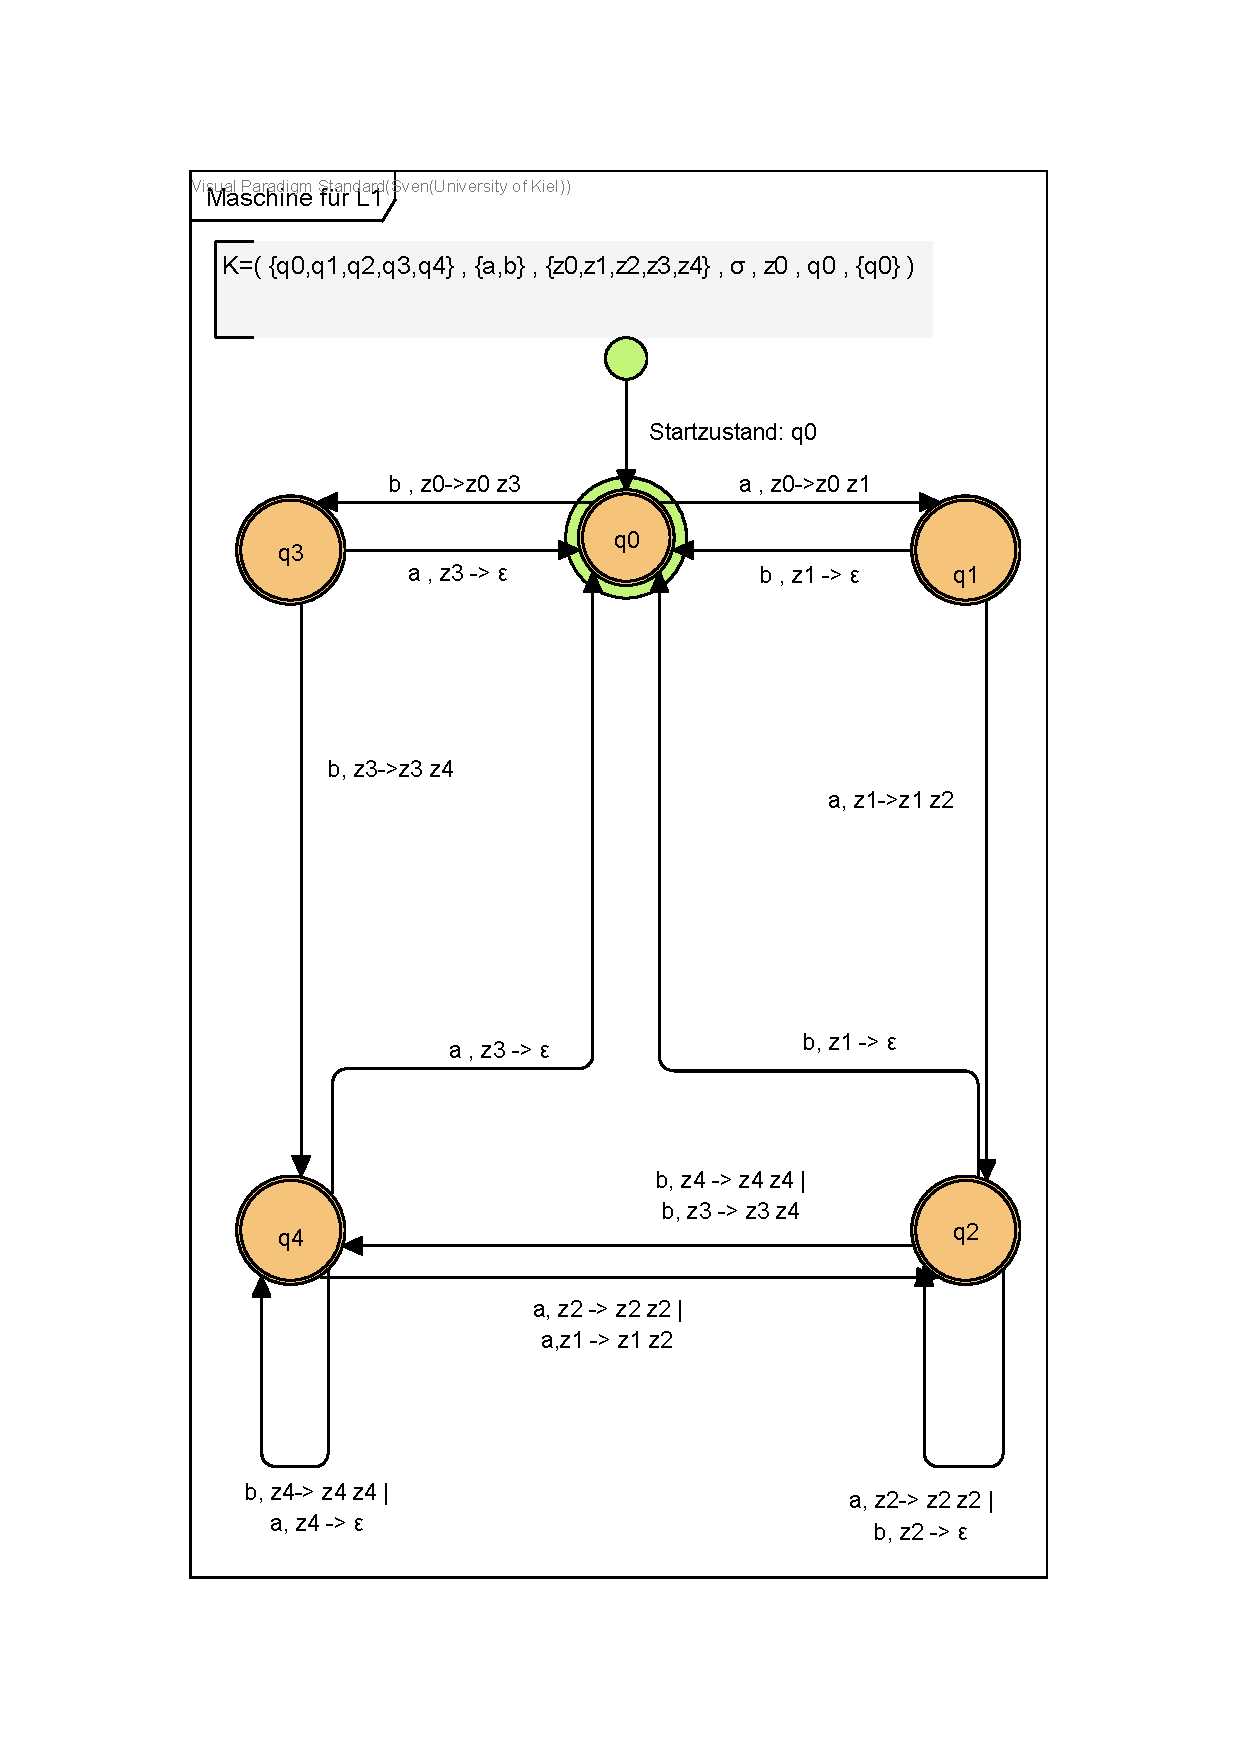
\includepdf[pages=-]{ErkenntL1H1.pdf}
	
\end{document}